\chapter{Exploratory Data Analysis}
\label{cha:eda}
%---------------------------------------------------------------------------


\section{Spotify Features}
\label{sec:spotifyfeatures}

\subsection*{Correlation Heatmap}
\label{sec:correlationheatmapsspotifyfeatures}

\begin{center}
\begin{figure}[H]
  \centering
  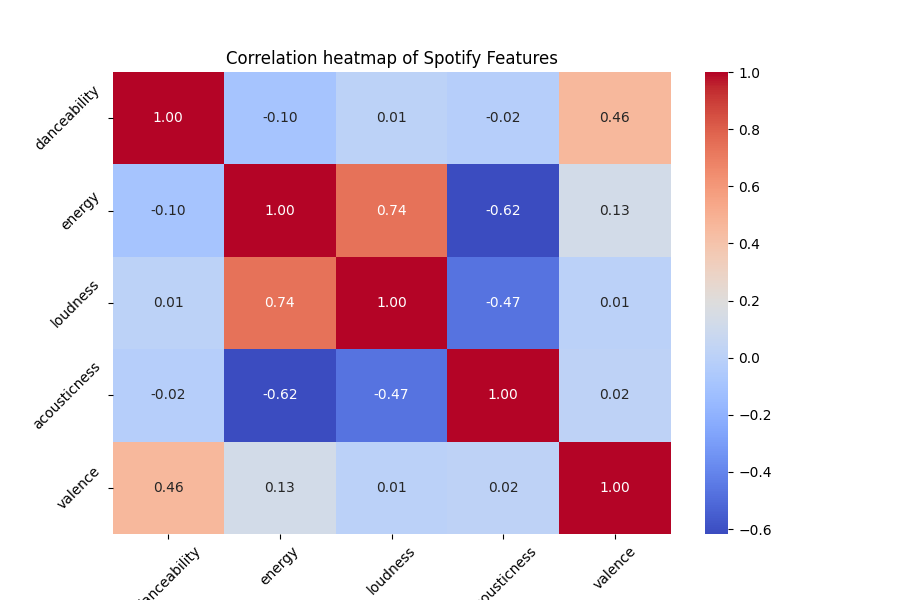
\includegraphics[width=5in]{img/corr_heatmap_spotify_features.png}
  \caption{Pearson's Correlation Heatmap of Spotify Features.}
  \label{Figure:fig_beh}
\end{figure}
\end{center}

\subsection*{Hierarchical Clustering}
\label{sec:hierarchicalclustering}

\begin{center}
\begin{figure}[H]
  \centering
  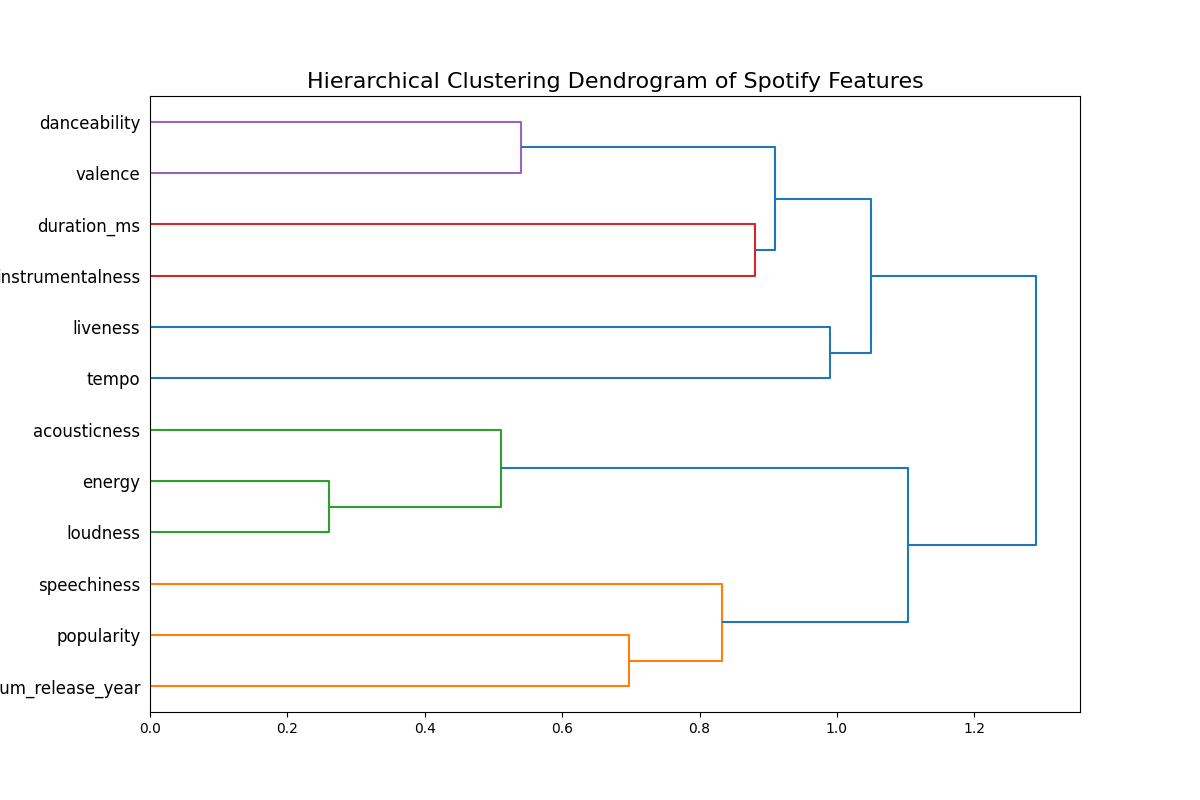
\includegraphics[width=4in]{img/dendrogram_spotify_features.png}
  \caption{Hierarchical Clustering of Spotify Features.}
  \label{Figure:dendrogram_spotify_features}
\end{figure}
\end{center}

\subsection*{Observations}
Spotify audio features show high level of correlation between each other, especially:
\begin{itemize}
  \item \textit{Energy} and \textit{Loudness}: A high correlation(0.74) suggest
    that energetic songs are typically louder;
  \item \textit{Danceability} and \textit{Valence}: high correlation between
    them indicates that songs perceived as positive and happy are usually more
    danceable;
  \item \textit{Energy} and \textit{Acousticness}: there is a strong negative
    correlation between those features, suggesting that high-energy tracks are
    less likely to have acoustic elements;
  \item The dendrogram(Fig.~\ref{Figure:dendrogram_spotify_features}) shows relations
    between features and allows us to compare which features correlate with
    each other. In addition to the relationships seen in the correlation
    heatmap, we observe that \textit{popularity} appears to have a weak
    correlation with \textit{release year} and \textit{speechiness}.

\end{itemize}


%---------------------------------------------------------------------------


\section{Lyrical Features}

\subsection*{Correlation Heatmap}
\label{sec:correlationheatmapsspotifyfeatures}

\begin{center}
\begin{figure}[H]
  \centering
  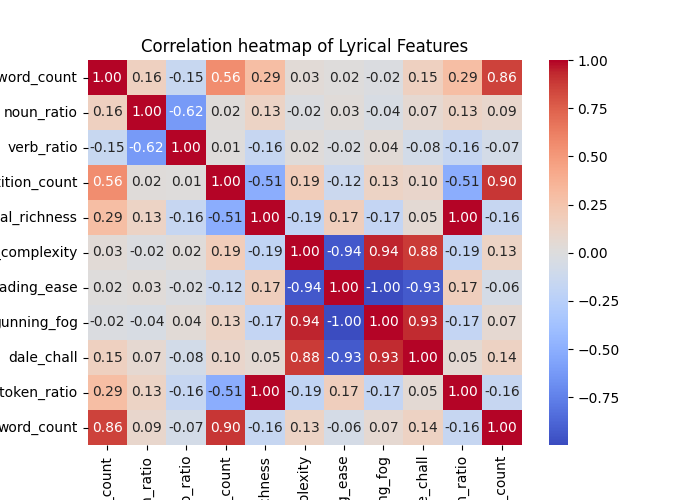
\includegraphics[width=5in]{img/corr_heatmap_lyrical.png}
  \caption{Pearson's Correlation Heatmap of Lyrical Features.}
  \label{Figure:fig_beh}
\end{figure}
\end{center}

\subsection*{Hierarchical Clustering}
\label{sec:hierarchicalclustering}

\begin{center}
\begin{figure}[H]
  \centering
  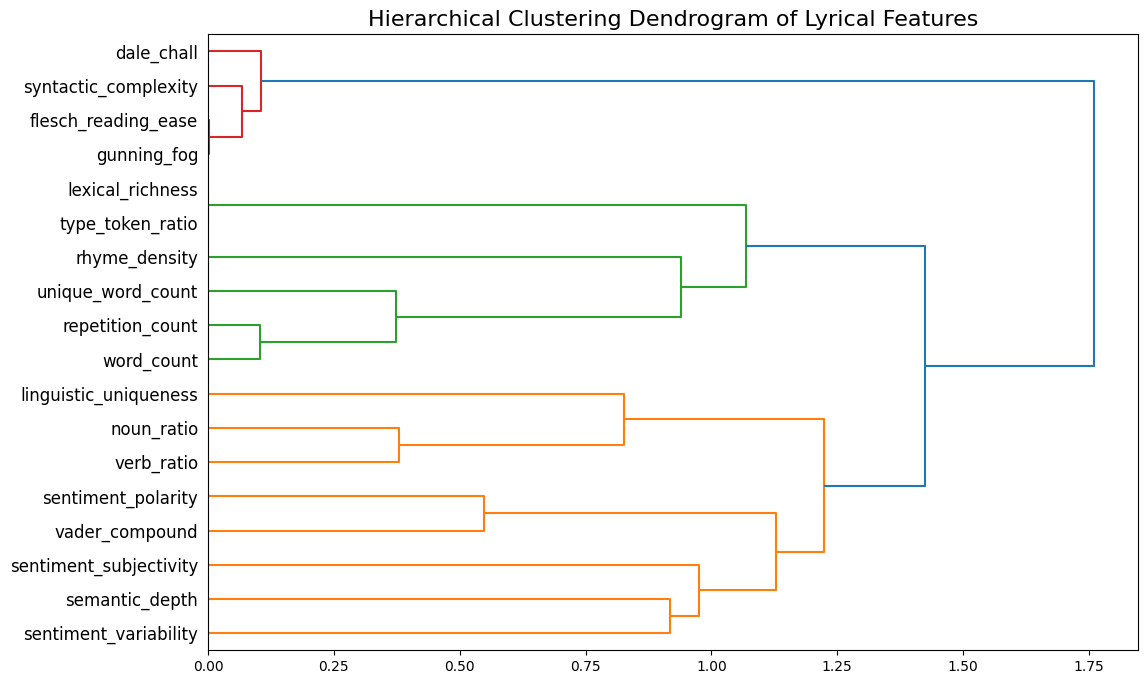
\includegraphics[width=4in]{img/dendrogram_lyrical.png}
  \caption{Hierarchical Clustering of Lyrical Features.}
  \label{Figure:dendrogram_spotify_features}
\end{figure}
\end{center}


\subsection*{Observations}

\begin{itemize}
  \item \textit{Flesch Reading Ease}, \textit{Gunning Fog} and \textit{Dale
    Chall} scores exhibit strong positive correlations, highlighting their
    shared focus on measuring lyrical complexity;
  \item \textit{Lexical Richness} correlates with \textit{Word Count},
    indicating that more lexically rich lyrics tend to have  greater variety
    of words;
  \item On the dendrogram we can distinguish three major clusters of features:
    \begin{itemize}
      \item \textbf{Lyrical Complexity Metrics} - \textit{Flesch Reading Ease},
        \textit{Gunning Fog}, \textit{Dale Chall} and \textit{Syntactic
        Complexity } quantify how difficult and complex the lyrics are;
      \item  \textbf{Lexical Features} - features such as \textit{Type-Token
        Ratio}, \textit{Lexical Richness} and \textit{Unique Word Count} form a
        cohesive cluster;
      \item \textbf{Sentiment-Related Features} - it includes \textit{Sentiment
        Polarity}, \textit{VADER Compound} and \textit{Semantic Depth}, which
        reflect emotional aspects of the lyrics.
    \end{itemize}
  \item Sentiment-related features are relatively closely grouped, suggesting a
    high level of interdependence.
\end{itemize}


%---------------------------------------------------------------------------
\section{Audio Features}

\subsection*{Correlation Heatmap}
\label{sec:correlationheatmapsspotifyfeatures}

\begin{center}
\begin{figure}[H]
  \centering
  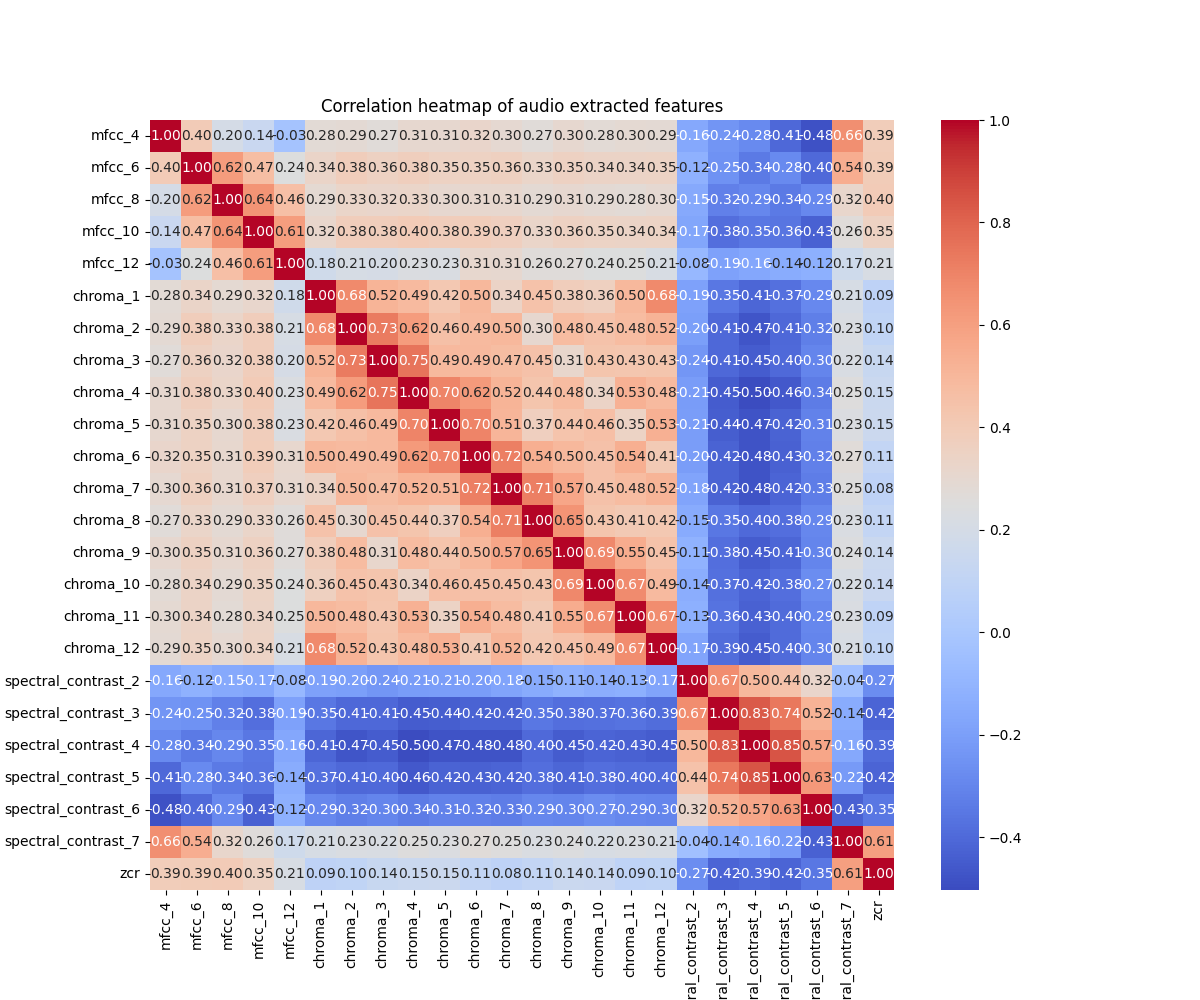
\includegraphics[width=5in]{img/corr_heatmap_audio.png}
  \caption{Pearson's Correlation Heatmap of Audio Features.}
  \label{Figure:fig_beh}
\end{figure}
\end{center}

\subsection*{Hierarchical Clustering}
\label{sec:hierarchicalclustering}

\begin{center}
\begin{figure}[H]
  \centering
  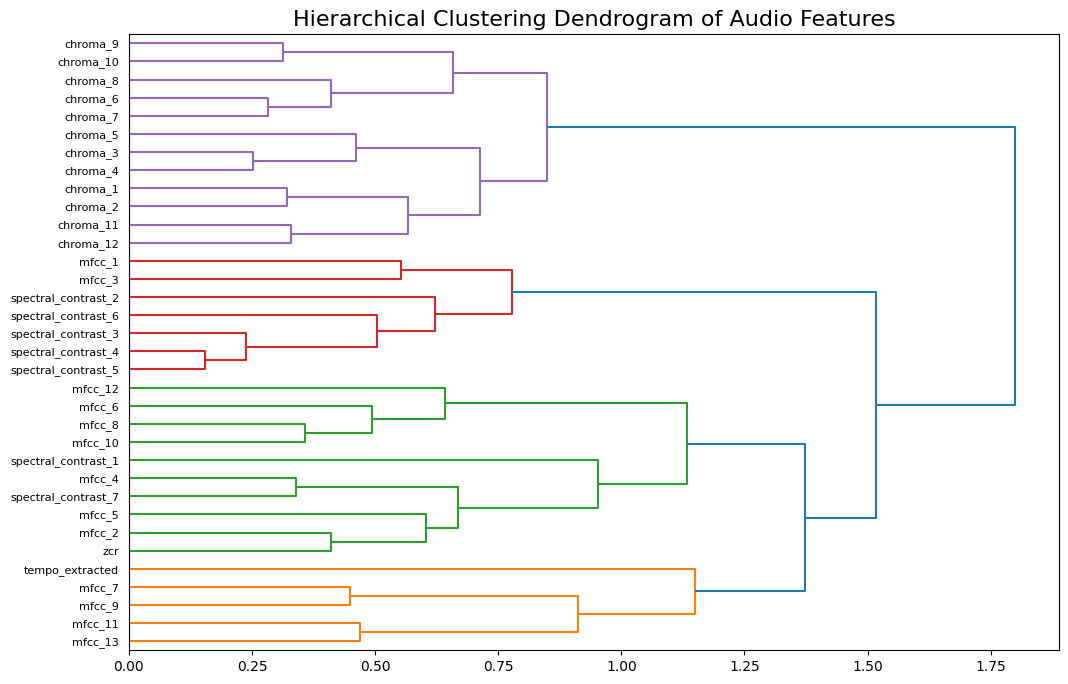
\includegraphics[width=4in]{img/dendrogram_audio.png}
  \caption{Hierarchical Clustering of Audio Features.}
  \label{Figure:dendrogram_spotify_features}
\end{figure}
\end{center}


\subsection*{Observations}
\begin{itemize}
  \item \textit{MFCC Features} are strongly correlated among themselves(e.g.
    \textit{mfcc\_4}, \textit{mfcc\_6}, \textit{mfcc\_8}, etc.);
  \item Similarily \textit{chroma} features show high correlation with each
    other, indicating that they capture similar aspects of audio tracks;
  \item \textit{spectral\_contrast} features show relatively small
    correlations with \textit{mfcc} and  \textit{chroma} features, indicating 
    their uniqueness;
  \item All \textit{chroma} features are grouped together in the same cluster
    on the dendrogram, supporting the conclusion drawn from the heatmap about
    strong correlations between them;
  \item \textit{zcr} and \textit{tempo\_extracted} are relatively independent;
  \item Some of the \textit{mfcc} and \textit{spectral\_contrast} features
    are to some degree correlated.
\end{itemize}

%---------------------------------------------------------------------------


\section{Empath Features}

\subsection*{Correlation Heatmap}
\label{sec:correlationheatmapsspotifyfeatures}

\begin{center}
\begin{figure}[H]
  \centering
  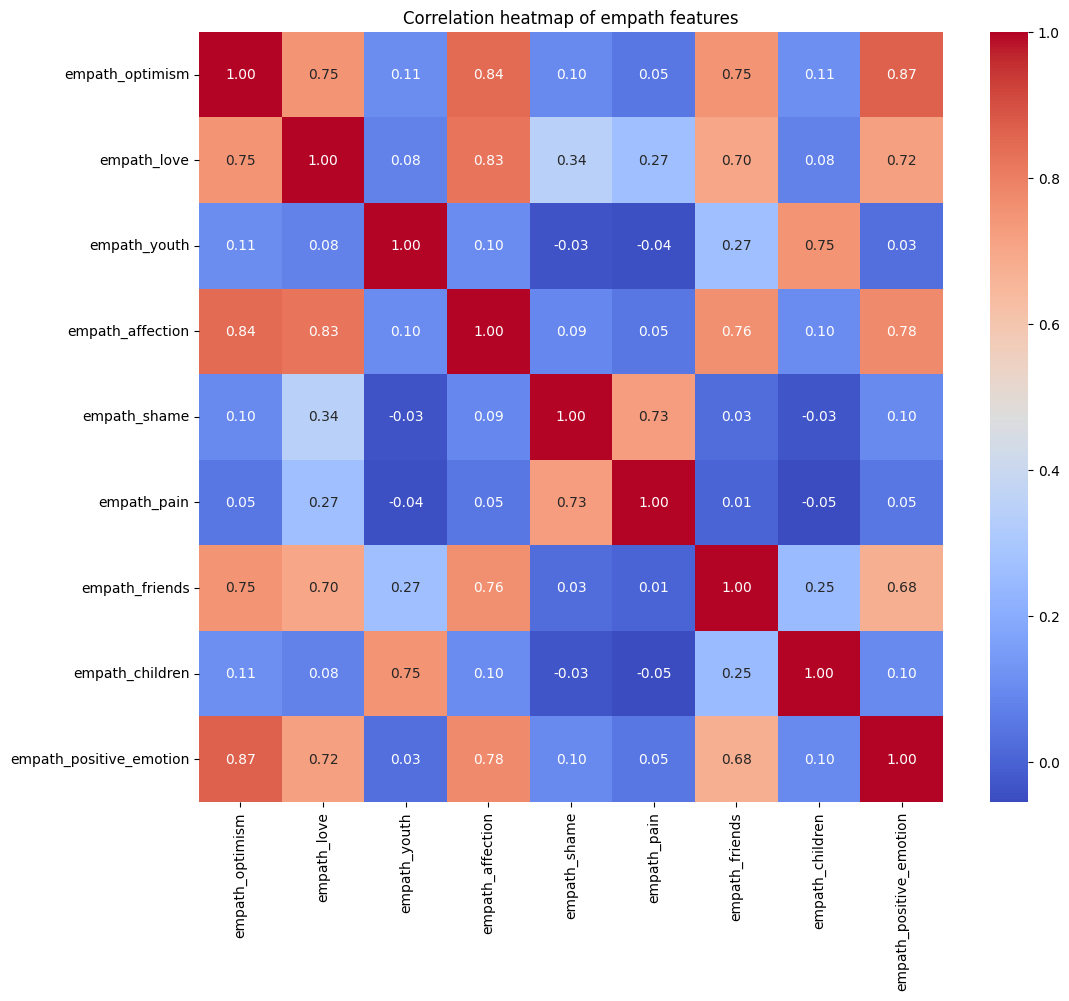
\includegraphics[width=5in]{img/corr_heatmap_empath.png}
  \caption{Pearson's Correlation Heatmap of Empath Features.}
  \label{Figure:fig_beh}
\end{figure}
\end{center}

\subsection*{Hierarchical Clustering}
\label{sec:hierarchicalclustering}

\begin{center}
\begin{figure}[H]
  \centering
  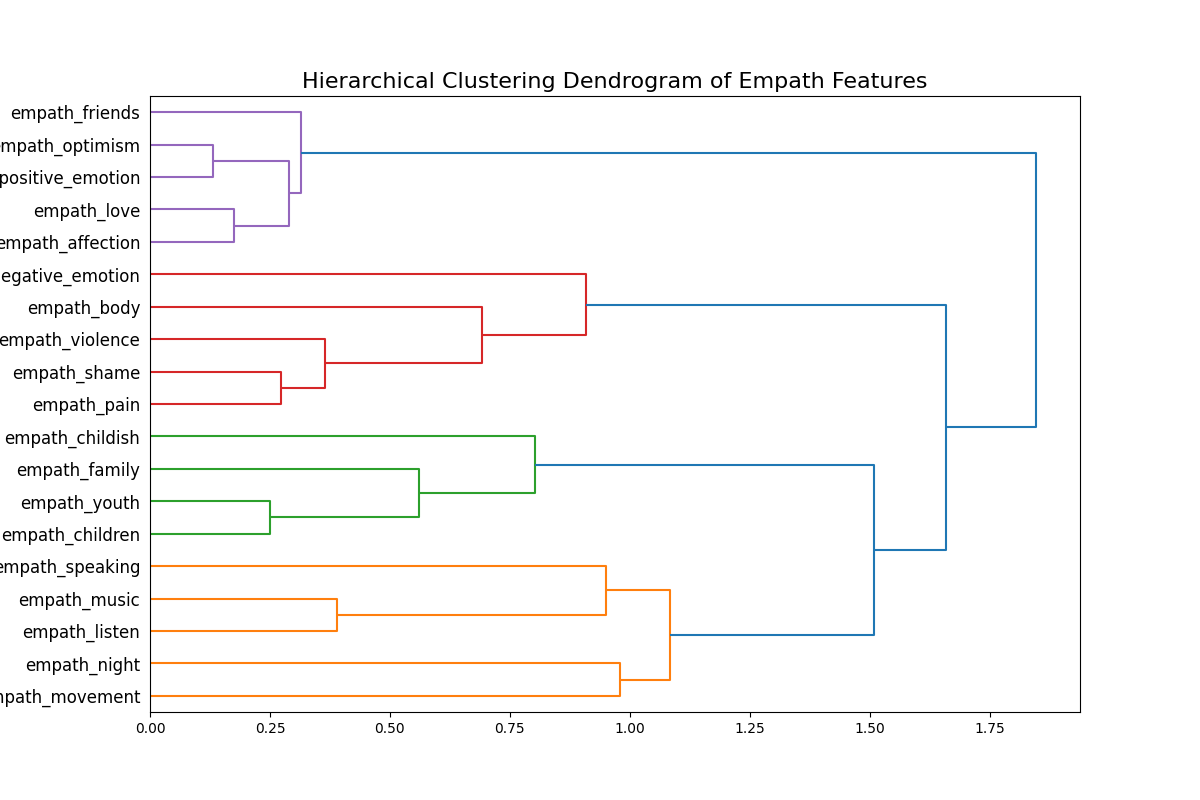
\includegraphics[width=4in]{img/dendrogram_empath.png}
  \caption{Hierarchical Clustering of Empath Features}
  \label{Figure:dendrogram_spotify_features}
\end{figure}
\end{center}


\subsection*{Observations}

\begin{itemize}
  \item \textbf{High Correlations Reflect Logical Groupings}: high correlation
    between features like \textit{empath\_optimism}, \textit{empath\_love} and
    \textit{empath\_affection} align with the intuitive understanding that
    these aspects are closely related;
  \item Observed patters in correlations confirm that Empath was designed to
    group semantically related concepts together;
  \item The visualizations align with the intended design of Empath as a tool
    for interpretable feature extraction.
\end{itemize}


%---------------------------------------------------------------------------

\section{Genre Analysis}

\subsection{Genre Similarity}

\begin{center}
\begin{figure}[H]
  \centering
  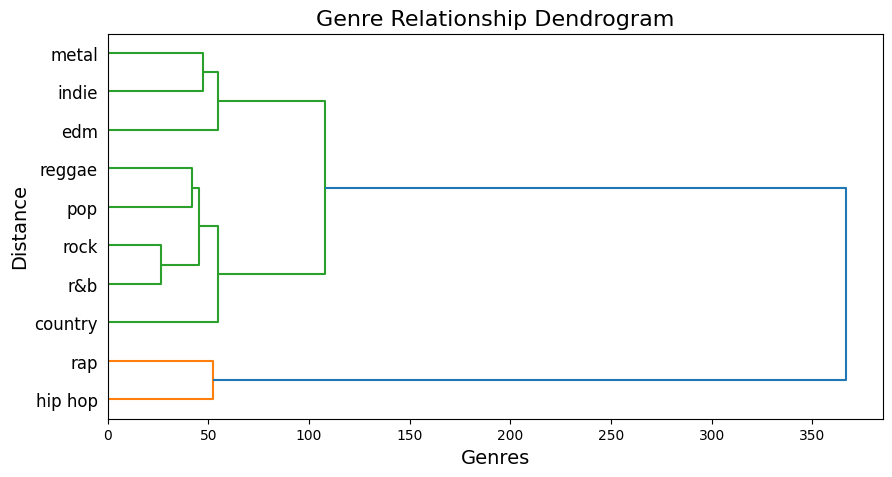
\includegraphics[width=5in]{img/genres_dendrogram.png}
  \caption{Hierarchical Clustering of Genres by lyrical and audio features.}
  \label{Figure:dendrogram_spotify_features}
\end{figure}
\end{center}

\begin{center}
\begin{figure}[H]
  \centering
  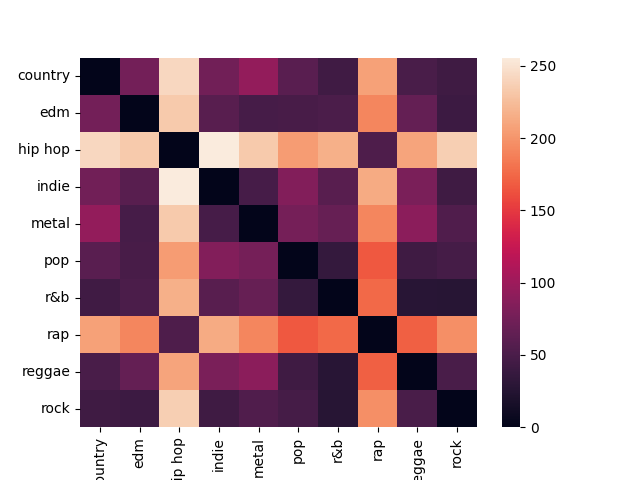
\includegraphics[width=4in]{img/genres_similarity_heatmap.png}
  \caption{Heatmap of euclidean distance of Genres calculated on lyrical and
  audio features.}
  \label{Figure:dendrogram_spotify_features}
\end{figure}
\end{center}

The dendrogram illustrates hierarchical clustering of genres based on their
lyrical and audio features. The similarities between genres align with their
general cultural and musical understandings, e.g. rap and hip hop are closely
related, indicating that they're quite similar. 

The heatmap further supports this observation. The euclidean distances of rap
and hip hop with other genres stand out as the highest, meaning that those two
genres are similar to each other and very different to all other genres
included in this study. 

Interestingly, genres such as metal and indie, while
distinct in sound, share some overlap in features, which is reflected on the
dendrogram.


\begin{center}
\begin{figure}[H]
  \centering
  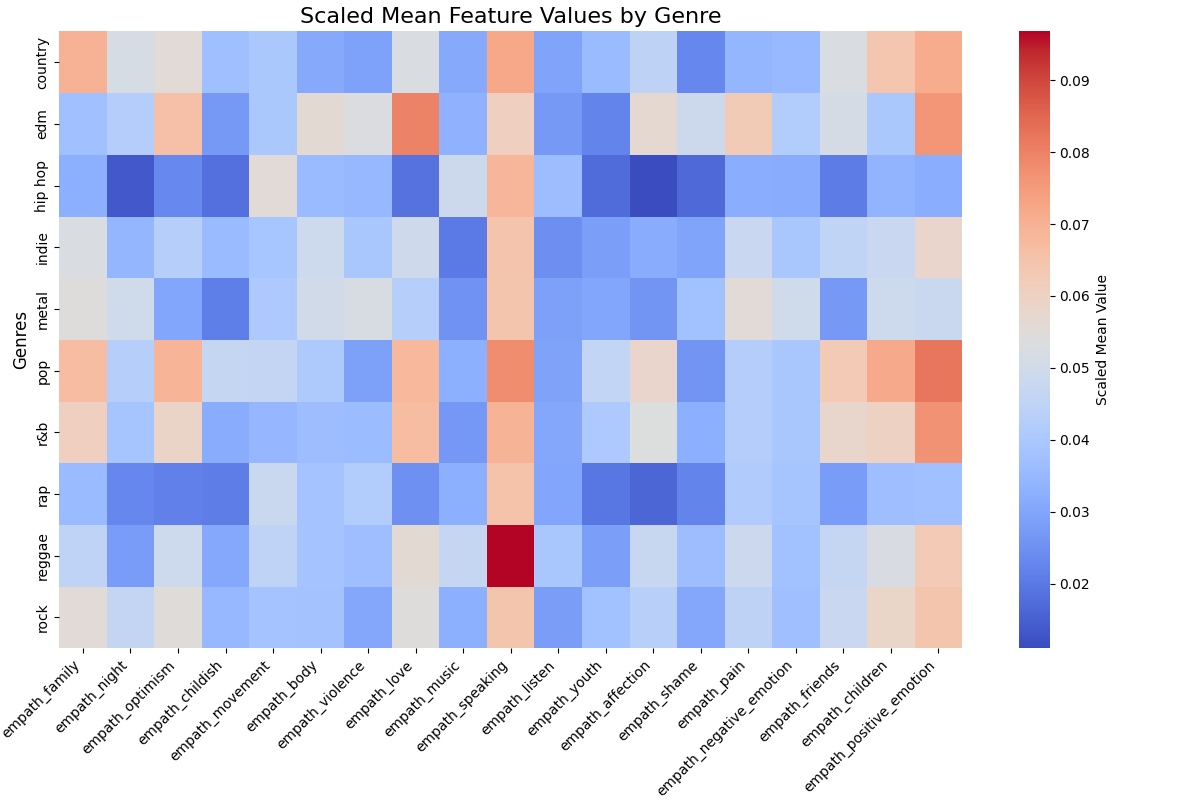
\includegraphics[width=6in]{img/heatmap_of_empath.png}
  \caption{Heatmap of mean values of empath features in each genre.}
  \label{Figure:heatmap_empath}
\end{figure}
\end{center}

The heatmap on figure Fig.~\ref{Figure:heatmap_empath} displays scaled mean
values of \textit{Empath features} for different musical genres. It visualizes
the thematic  differences in their lyrics. It can be observed that:
\begin{itemize}
  \item \textbf{Country} music lyrics often involve topics related to family,
    love and  positive emotions. It seems to align well with genre's tendency
    to narrate personal, heartfelt and often nostalgic stories;
  \item \textbf{EDM} lyrics seem to often talk about love and optimism;
  \item For both \textbf{Hip Hop} and \textbf{Rap} according to Empath  the
    most prominent topic is \textit{speaking};
  \item For \textbf{Metal} high values in \textit{negative emotion} and
    \textit{pain} reflects the genre's focus on intense, darker themes;
  \item Higher values in \textit{love} and \textit{positive emotion}
    aligns with \textbf{Pop} music’s focus on themes of love and relationships;
  \item High values in \textit{friends} and \textit{optimism} categories
    reflect \textbf{Reggae's} focus on positivity, social connection, and
    uplifting messages.
\end{itemize}

\subsection{Lyrical Similarity Based on Embeddings}
\begin{center}
\begin{figure}[H]
  \centering
  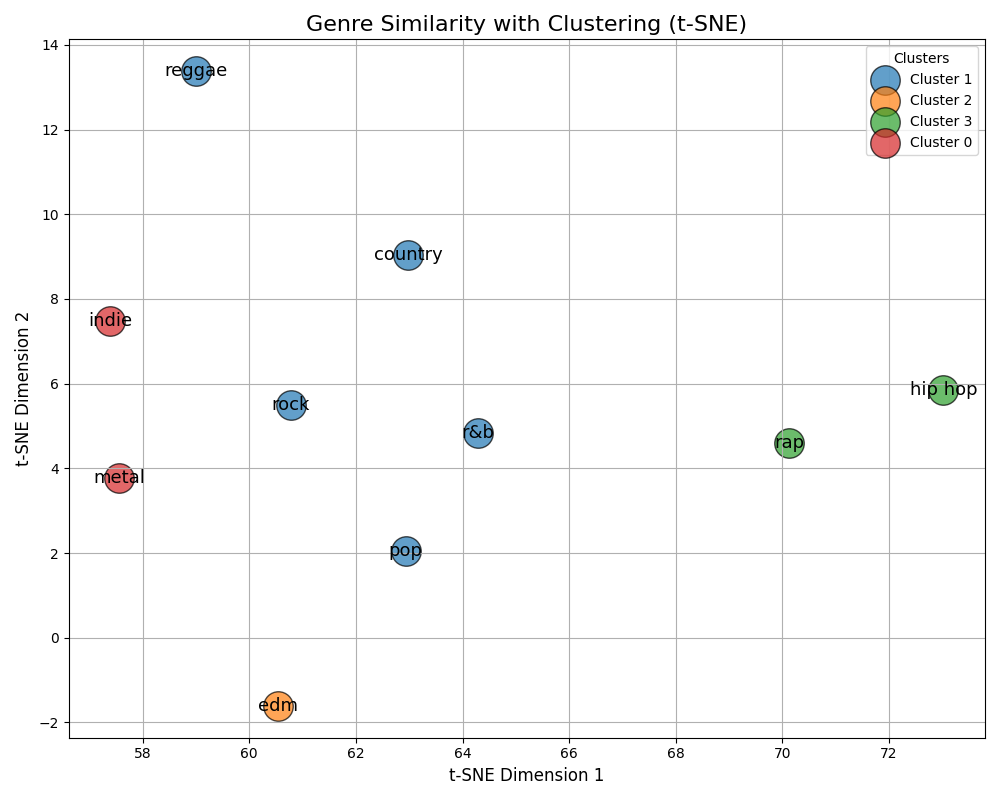
\includegraphics[width=6in]{img/tsne_genres.png}
  \caption{Lyrical Genre Similarity Based on Embeddings.}
  \label{Figure:dendrogram_spotify_features}
\end{figure}
\end{center}
\textbf{t-SNE (t-Distributed Stochastic Neighbor Embedding)} is a statistical method for
visualizing high-dimensional data by reducing it to lower- dimensional spaces,
while preserving the relative distances and similarities between data points as
much as possible. It was applied to the euclidean distance matrix of mean
standardized Word2Vec and TF-IDF embeddings for each genre in order to
visualize lyrical similarities between different genres.

\textbf{K-means clustering} was applied as well on the mean standardized embeddings per
genre with optimal number of clusters determined using the elbow method(which
suggested four clusters). This operation clusters the most similar genres
together, additionally enhancing the visualization.


\begin{itemize}
  \item \textit{Hip hop} and \textit{rap} form a distinct cluster, indicating
    strong lyrical and thematic similarity and dissimilarity with other genres;
  \item \textit{Reggae} is slightly separate from other genres but still
    belongs to the cluster that includes \textit{rock}, \textit{pop},
    \textit{country}, and \textit{R\&B}, suggesting moderate similarity in
    lyrical and thematic content of songs belonging to those genres;
  \item \textit{Metal} and \textit{indie} are closely positioned, sharing
    overlapping themes and forming a  separate cluster;
  \item \textit{EDM} is positioned furthest from other genres and belongs to
    its own cluster, highlighting its unique lyrical and thematic style.
\end{itemize}

\subsection{Top Genre Characteristics}
\begin{center}
\begin{figure}[H]
  \centering
  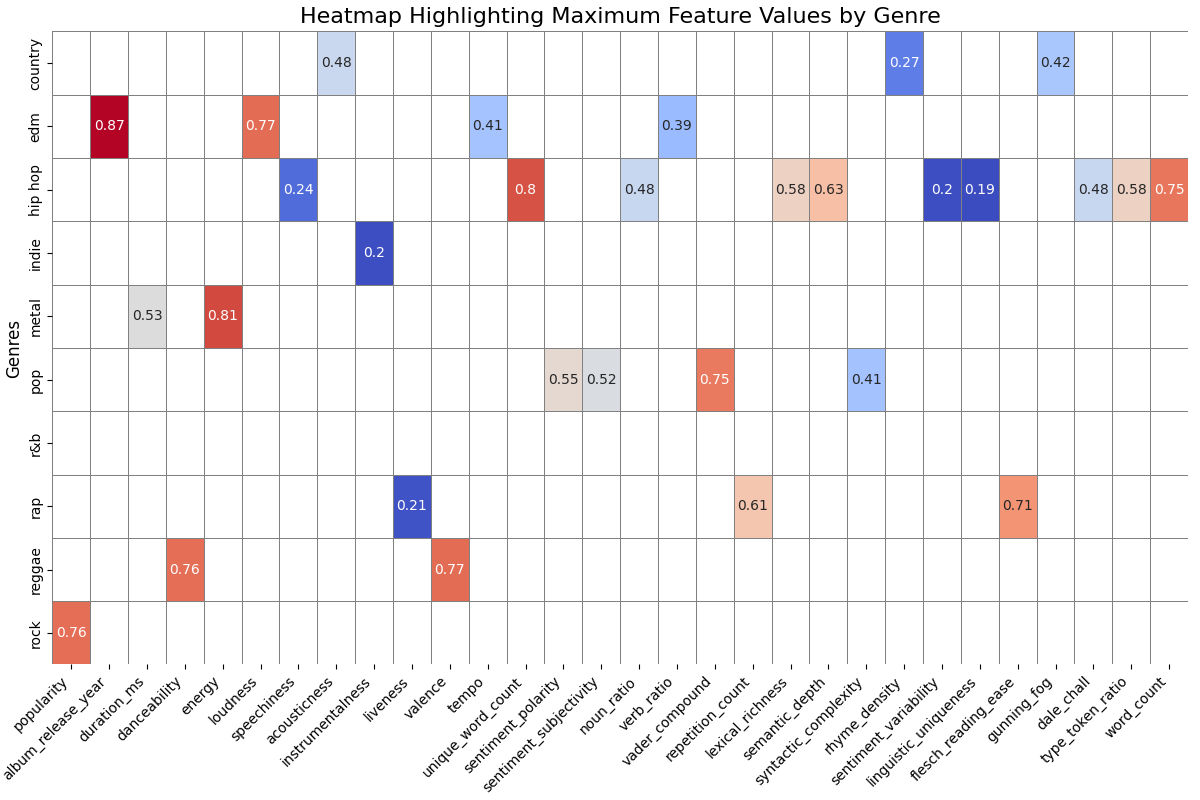
\includegraphics[width=6in]{img/heatmap_max_feature_values_by_genre.png}
  \caption{Heatmap highlighting the maximum feature values across genres.}
  \label{Figure:dendrogram_spotify_features}
\end{figure}
\end{center}
Each filled cell represents the genre that exhibits the highest mean value for
the corresponding feature, calculated using scaled feature values. This
visualization emphasizes distinctive characteristics of each genre, and allows
to see ``in  which genre the feature achieved its highest mean``.

\begin{itemize}
  \item \textbf{Country}: Highest in acousticness and rhyme density;
  \item \textbf{EDM}: Dominated in tempo, loudness, and featured the most
    recent songs;
  \item \textbf{Hip Hop}: Excelled in unique word count, lexical richness, and
    semantic depth;
  \item \textbf{Metal}: Stood out for energy and longer song durations;
  \item \textbf{Pop}: Showed the highest positivity (VADER compound) and
    subjectivity in lyrics;
  \item \textbf{Rap}: Highest in repetition count and reading ease;
  \item \textbf{Reggae}: Highlighted by high valence and danceability;
  \item \textbf{Rock}: Scored highest in in popularity.
    
\end{itemize}

\begin{center}
\begin{figure}[H]
  \centering
  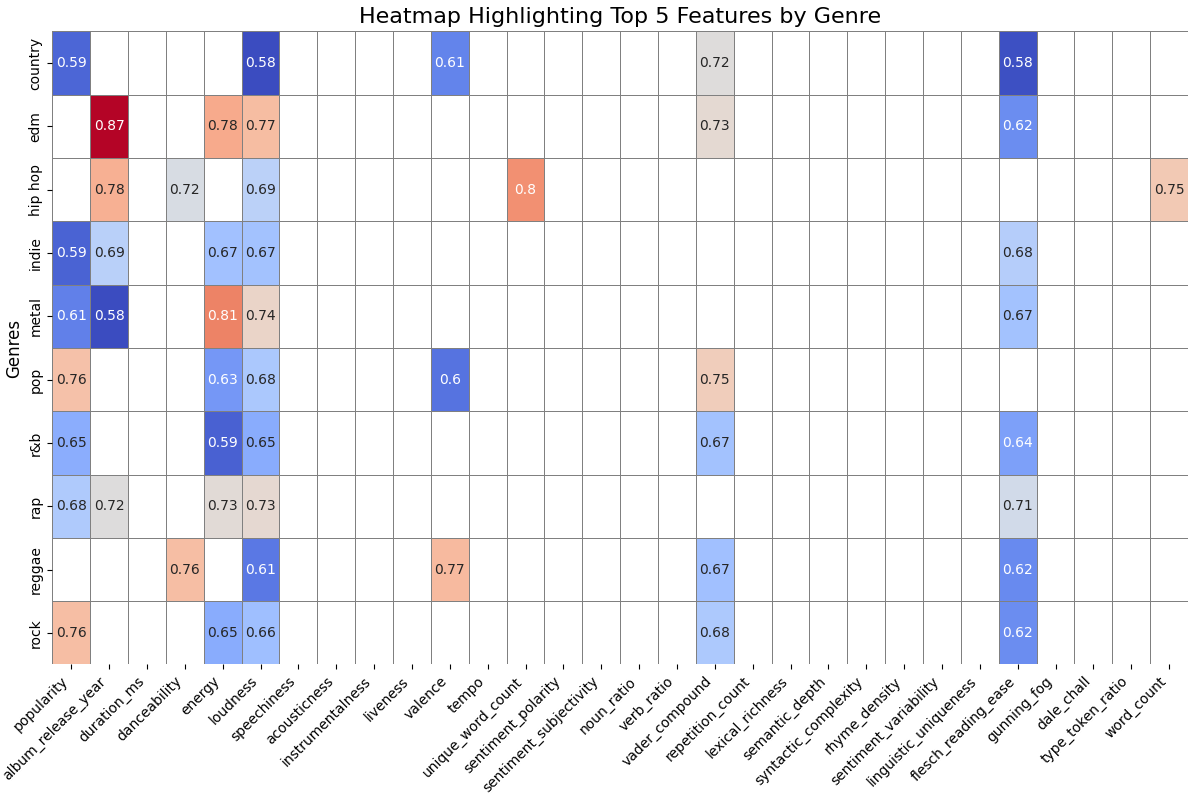
\includegraphics[width=6in]{img/heatmap_top_feature_values_by_genre.png}
  \caption{Heatmap highlighting the top 5 features by genre. Each filled cell
    represents one of the five highest mean feature values for a given genre,
    calculated on scaled data. This visualization shows what are ``the top 5
    most characteristic properties of each genre``. }
  \label{Figure:dendrogram_spotify_features}
\end{figure}
\end{center}

Lastly, we switch perspectives, focusing not on individual features but instead
examining each genrer to identify the top 5 features that characterize it. Each
filled cell in that heatmap shows one of the five most prominent
characteristics exhibited by that genre.

